\chapter{La complessità spaziale} \label{ch:capitolo16}
\subsection{Macchina di turing a piu' strati}
\begin{figure}[htp]
    \centering
    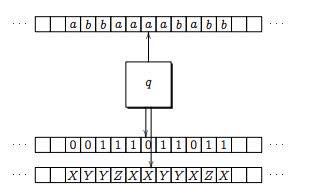
\includegraphics[scale=0.6]{tesi_stile/img/f1cap16.png}
\end{figure}
Una macchina di Turing M a più nastri è composta da:
\begin{itemize}
    \item un’unità di controllo a stati finiti
    \item un nastro $N_0$ di input-output di lunghezza infinita con relativa testina
    \begin{itemize}
        \item I nastri sono suddivisi in celle, e ogni cella contiene un simbolo di un certo alfabeto A oppure il simbolo bianco \#.
    \end{itemize}
    \item Inizialmente, il nastro di input-output $N_0$ contiene l’input, la testina è sul simbolo più a sinistra, lo stato è $q_0$, gli altri nastri sono vuoti.
    \item Ogni successiva mossa di M è determinata da
    \begin{itemize}
        \item stato
        \item simboli letti dalle testine sugli m nastri
    \end{itemize}
    \item consiste in: 
    \begin{itemize}
        \item aggiornare lo stato
        \item modificare i simboli esaminati su ogni nastro
        \item spostare in ogni nastro la testina di un passo verso destra, verso sinistra o lasciarla ferma
    \end{itemize}
\end{itemize}
\textbf{Definizione}\\
Una Macchina di Turing a m nastri è una quadrupla $M = (Q, A, \sigma, q_0)$,
dove:
\begin{itemize}
    \item Q è un insieme finito di stati 
    \item A è un alfabeto, cui si aggiunge il simbolo bianco \#
    \item $\sigma$ è una funzione parziale da Q × $(A$ U $\{\#\})^m$ a 
    
    $Q x (A$ U $\{\#\}) m x \{-1, 0, 1\}^m$ , chiamata funzione di transizione
    
    \item $q_0 \in Q$ è lo stato iniziale
\end{itemize}
Le (2m + 1)-tuple
\begin{center}
    $(q, a_1 ..., a_m, q', a^{'}_1,..., a^{'}_m , x_1,..., x_m)$
\end{center}
tali che\\\\
$\sigma(q, a_1, ... , a_m )$ $= (q', a^{'}_1,..., a^{'}_m , x_1,..., x_m)$
\\\\sono dette le istruzioni di M.
\newpage
\textbf{Esempio}\\
Una macchina di Turing a due nastri che accetta le palindrome\\\\
\textbf{Startegia}
\begin{itemize}
    \item Copiamo l’input, capovolto, sul nastro ausiliario
    \item Riportiamo la testina del nastro di input/output all’inizio dell’input
    \item Esaminiamo i due nastri verificando se contengono la stessa parola
\end{itemize}
\begin{figure}[htp]
    \centering
    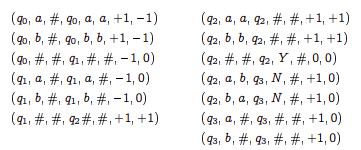
\includegraphics[scale=0.8]{tesi_stile/img/foto2cap16.png}
\end{figure}
\textbf{Osservazione}\\
Con due nastri, il tempo necessario alla verifica è 3n, con un nastro,$n(n-1)/2$
\subsection{Equivalenza tra modelli}
\textbf{Teorema}\\
Per ogni macchina di Turing M$=(Q, A, \sigma, q_0)$ con m nastri ausiliari, esiste una macchina di Turing $M'=(Q', A', \sigma', q^{'}_0)$ tale che
\begin{itemize}
    \item per ogni linguaggio L $\subseteq$ A, L è accettato o deciso da M se e solo se lo è da M'
    \item per ogni funzione $f : A* \mapsto A*$, f è calcolata da M se e solo se lo è da M'
\end{itemize}
\newpage
\subsection{Dimostrazione}
\begin{figure}[htp]
    \centering
    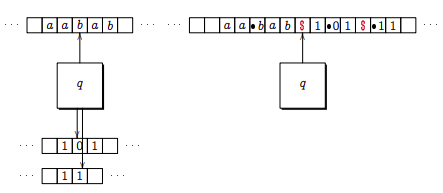
\includegraphics[scale=0.6]{tesi_stile/img/foto3cap16.png}
\end{figure}
\subsection{Complessità spaziale}
Valutare la quantità di memoria richiesta per la risoluzione di un problema
\begin{center}
    Il massimo numero di celle visitate dalla macchina di Turing nelle computazioni convergenti su input di lunghezza $<=$ n ?
\end{center}
Sarebbe sempre $>=$ n\\\\
\textbf{Esempio}\\
Per sommare due interi (espressi in binario) è necessario tenere traccia del
riporto: un solo bit, indipendentemente dalla dimensione dell’input.
\\È opportuno distinguere
\begin{itemize}
    \item lo spazio necessario per l’input
    \item lo spazio usato dallo sviluppo della computazione
\end{itemize}
\subsection{Il modello}
Macchina di Turing a piu' nastri:
\begin{itemize}
    \item un nastro di sola lettura su cui collocare l’input
    \item un nastro ausiliario di lavoro su cui svolgere la computazione
    \item un eventuale terzo nastro di sola scrittura, da usare una sola volta per l’output.
\end{itemize}
\textbf{Definizione}\\
La complessità spaziale di una macchina di Turing deterministica M (come sopra) è la funzione $s_M(n)$ che associa ad ogni naturale n il numero massimo di quadri impiegato da M sul nastro di lavoro nelle computazioni convergenti su input di lunghezza $<=$ n.
\subsection{Il modello non deterministico}
\textbf{Definizione}
\\Sia M una macchina di Turing non deterministica (come sopra).
\\Per ogni parola w accettata da M, denotiamo con $s_w$ il minimo numero di quadri impiegato sul nastro di lavoro da una computazione convergente di M su input w.
\\Si dice complessità spaziale di M la funzione $s_M : N \mapsto N$ definita come segue: per ogni $n \in N$,
\begin{center}
    $s_M(n) = max\{sw | w accettata da M, l(w) <= n\}.$
\end{center}
\textbf{Qualche osservazione}\\
\begin{center}
    $s_M (n) <= c_M (n)$
\end{center}
Invero, in una computazione di t passi, si possono visitare al più t celle sul
nastro di lavoro.
\\Viceversa
\begin{center}
    $c_M (n) = n * 2^{O(s_M(n))}$
\end{center}
\subsection{Dimostrazione}
Una configurazione istantanea di una macchina di Turing in una computazione convergente su un input di lunghezza n è determinata da
\begin{center}
    \item Lo stato (k = Card Q possibilità)
    \item La posizione della testina sul nastro di input (n possibili posizioni)
    \item La posizione della testina sul nastro di lavoro ($s_M (n)$ possibili posizioni)
    \item Il contenuto del nastro di lavoro $(d^{sM(n)}$ possibilità, con d $=$ 1 $+$ Card A)
\end{center}
Pertanto il numero di tali configurazioni è maggiorato da\\
\begin{figure}[htp]
    \centering
    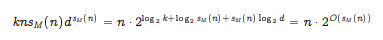
\includegraphics[scale=0.8]{tesi_stile/img/foto4cap16.png}
\end{figure}
\\In una computazione convergente, una configurazione istantanea non può ripetersi.
\\Ne segue l’asserto
\subsection{Classi di complessità spaziale}
\textbf{PSPACE} è la classe dei problemi di decisione S che sono accettati da
macchine di Turing (deterministiche) M tali che $s_M(n) = O(n^k)$ per qualche intero positivo k.
\\\textbf{LOGSPACE} (o, brevemente, L) è la classe dei problemi di decisione S che sono accettati da macchine di Turing (deterministiche) M tali che $s_M(n) = O(\log n).$\\\\
\textbf{Osservazione}
\begin{center}
    $L \subseteq P \subseteq PSPACE \subseteq PEXP$.
\end{center}
Si ha L $\neq$ PSPACE e quindi vale almeno una delle disuguaglianze
\begin{center}
    $L \neq P oppure P\neq PSPACE$
\end{center}
\textbf{Congettura}\\
\begin{center}
     $L \neq P$
\end{center}
\newpage
\subsection{Classi non deterministiche}
\textbf{Definizione}\\
\textbf{PSPACE} è la classe dei problemi di decisione S che sono accettati da
macchine di Turing (deterministiche) M tali che $s_M(n) = O(n^k)$ per qualche intero positivo k.
\\\textbf{LOGSPACE} (o, brevemente, NL) è la classe dei problemi di decisione S che sono accettati da macchine di Turing (deterministiche) M tali che $s_M(n) = O(\log n).$\\\\
\textbf{Osservazione}\\
Si ha
\begin{itemize}
    \item PSPACE $\subseteq$ NPSPACE
    \item L $\subseteq$ NL
    \item NP $\subseteq$ NPSPACE
\end{itemize}
\subsection{Il grafo delle computazioni}
Le computazioni di una macchina di Turing M su un particolare input w
sono descritte dal grafo diretto G(M, w) definito da
\begin{itemize}
    \item I vertici di G(M, w) sono le configurazioni istantanee di M nelle computazioni convergenti su input w e un ulteriore vertice t(M, w)
    \item Le frecce connettono le configurazioni consecutive (legate dalla relazione $\vdash$M ). 
\\Inoltre, ci sono frecce da tutte le configurazioni di arresto a t(M, w).
\end{itemize}
\textbf{Osservazione}\\
Come si è visto, il numero degli stati di G(M(w)) è $2^{O(s_M(n))}$, ove $n=l(w)$.
Il medesimo limite vale per il numero delle frecce.
\\Inoltre ogni vertice può essere descritto con $O(s_M (n) + \log n)$ bit di
informazione